\begin{frame}
  \frametitle{Simple \vs complex settings -- QITL-1 revisited}

  \begin{itemize}
  \item \citet{Arppe:Jarvikivi:02,Arppe:Jarvikivi:07}
  \item \textit{Person} (\textsc{first person singular} or not) and
    \textit{Countability} (\textsc{collective} or not) of \textsc{agent/subject} of
    Finnish verb synonym pair \textit{mietti{\"a}} \vs \textit{pohtia}
    `think, ponder':
  \end{itemize}

  \begin{center}\scriptsize
    \begin{tabular}{ c  c || c || c  c}
      \hline
      \multicolumn{2}{c||}{Forced-choice}                     & Frequency           & \multicolumn{2}{c}{Acceptability}    \\
      Dispreferred                          & Preferred       & (relative)          & Unacceptable                          & Acceptable       \\ \hline \hline
      \multicolumn{1}{c|}{$\varnothing$}    & mietti{\"a}+SG1 & Frequent            & \multicolumn{1}{c|}{$\varnothing$}    & mietti{\"a}+SG1  \\
      \multicolumn{1}{c|}{}                 & pohtia+COLL     &                     & \multicolumn{1}{c|}{}                 & pohtia{\"a}+COLL \\ \hline
      \multicolumn{1}{c|}{mietti{\"a}+COLL} &                 &                     & \multicolumn{1}{c|}{}                 &                  \\
      \multicolumn{1}{c|}{pohtia+SG1}       & $\varnothing$   & Rare                & \multicolumn{1}{c|}{mietti{\"a}+COLL} & pohtia+SG1       \\
      \hline
    \end{tabular}
  \end{center}
\end{frame}

\begin{frame}[c]
  \frametitle{QITL-1 through the lens of NDL}

  \centering\ungap[1]
  \only<beamer:1| handout:0>{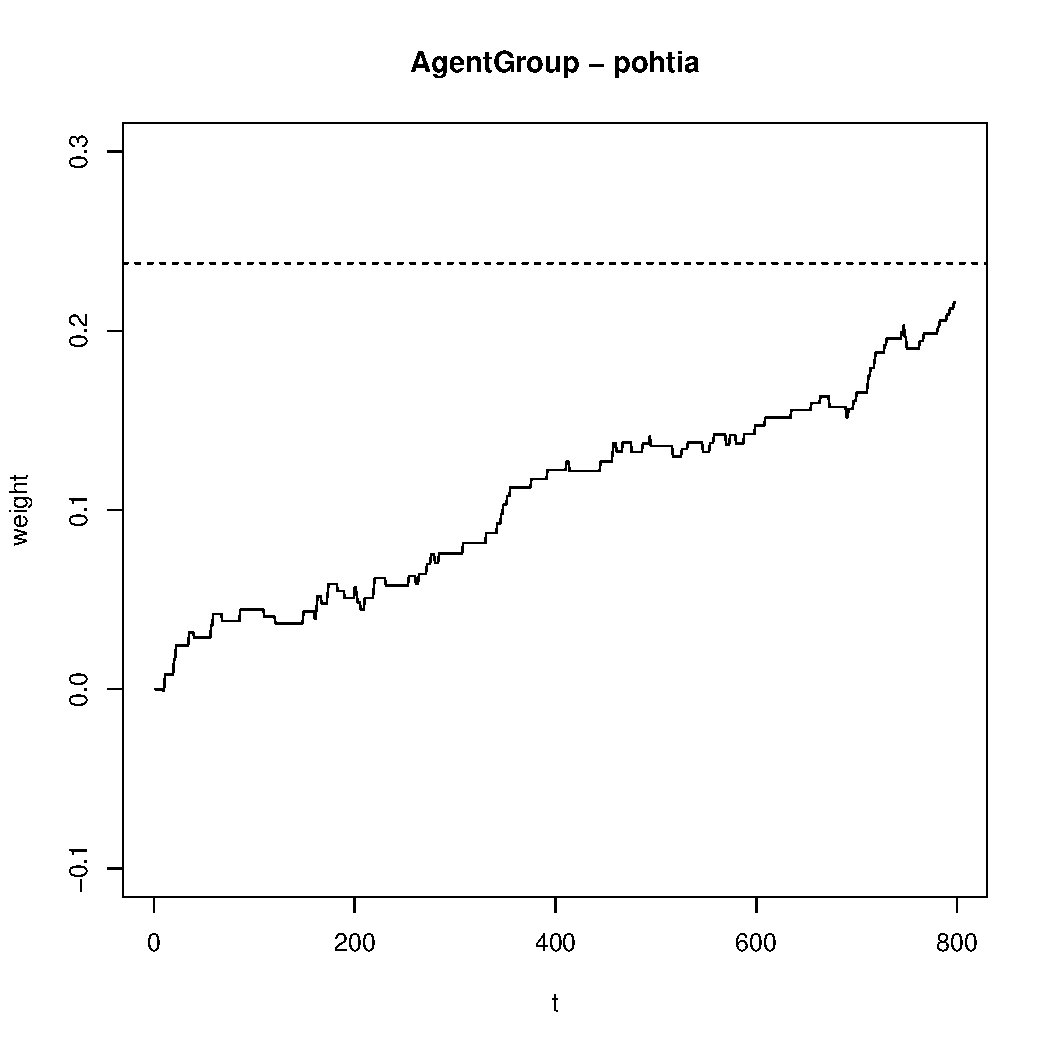
\includegraphics[width=8cm]{{{img/think.qitl1.AgentGroup_pohtia_RW_vs_D}}}}%
  \only<beamer:2| handout:0>{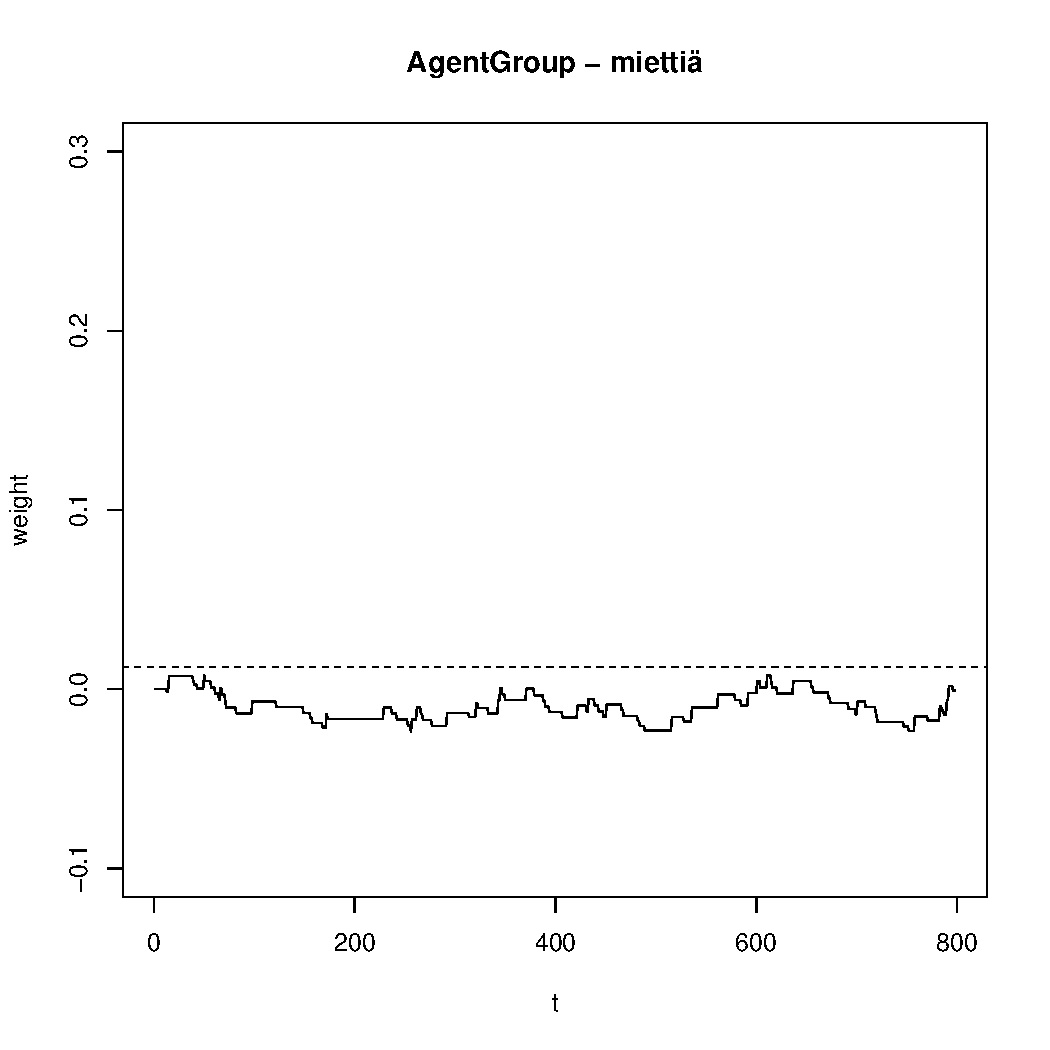
\includegraphics[width=8cm]{{{img/think.qitl1.AgentGroup_miettia_RW_vs_D}}}}%
  \only<beamer:3| handout:0>{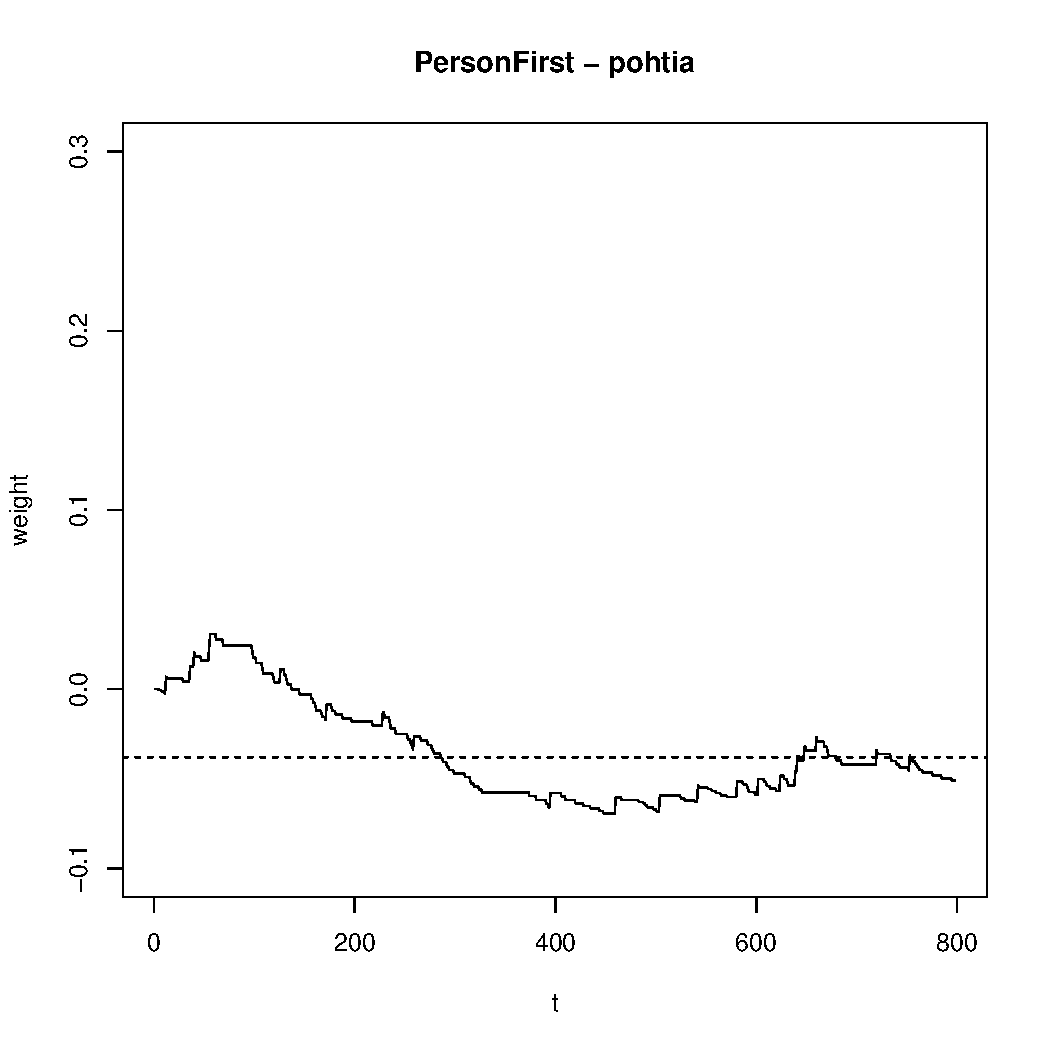
\includegraphics[width=8cm]{{{img/think.qitl1.PersonFirst_pohtia_RW_vs_D}}}}%
  \only<beamer:4| handout:0>{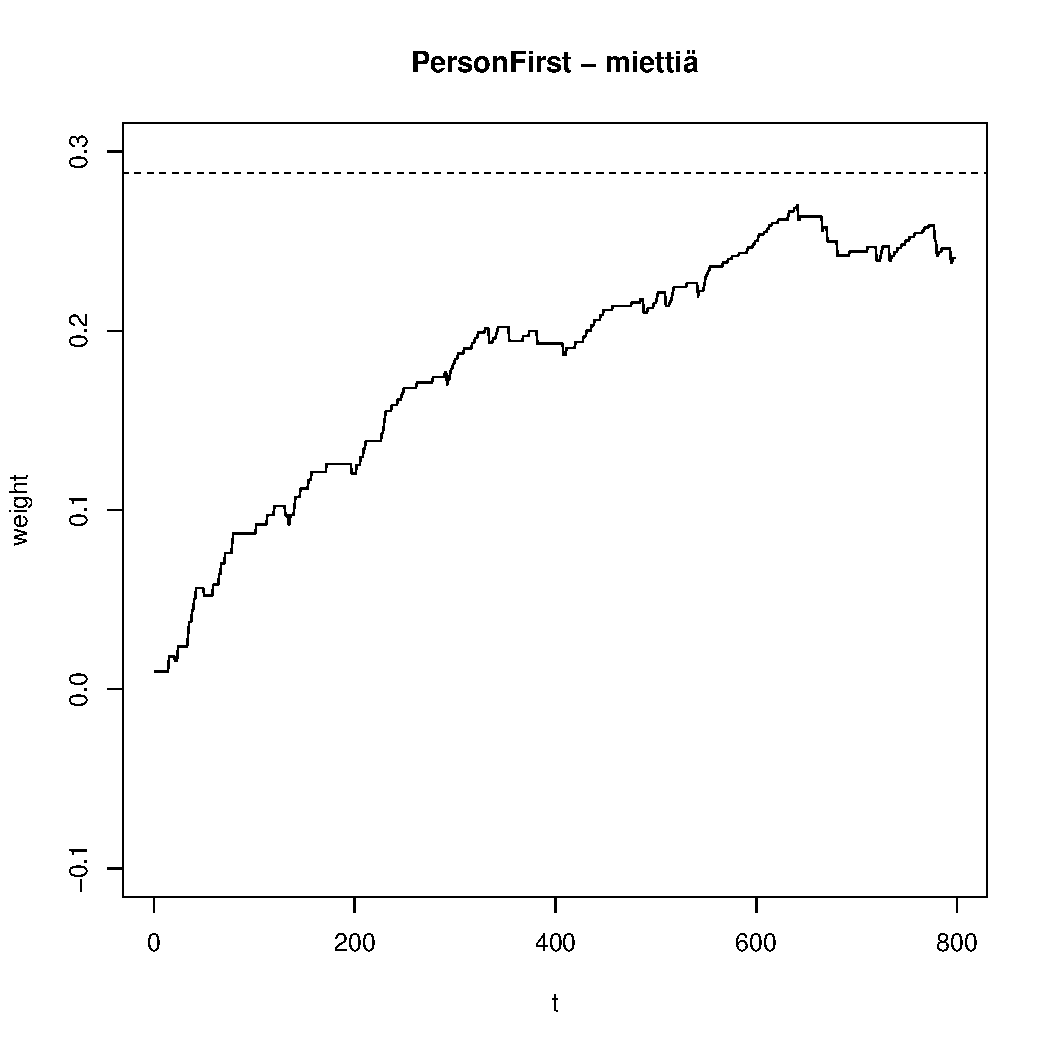
\includegraphics[width=8cm]{{{img/think.qitl1.PersonFirst_miettia_RW_vs_D}}}}%
  \only<beamer:0| handout:1>{%
    \begin{tabular}{cc}
      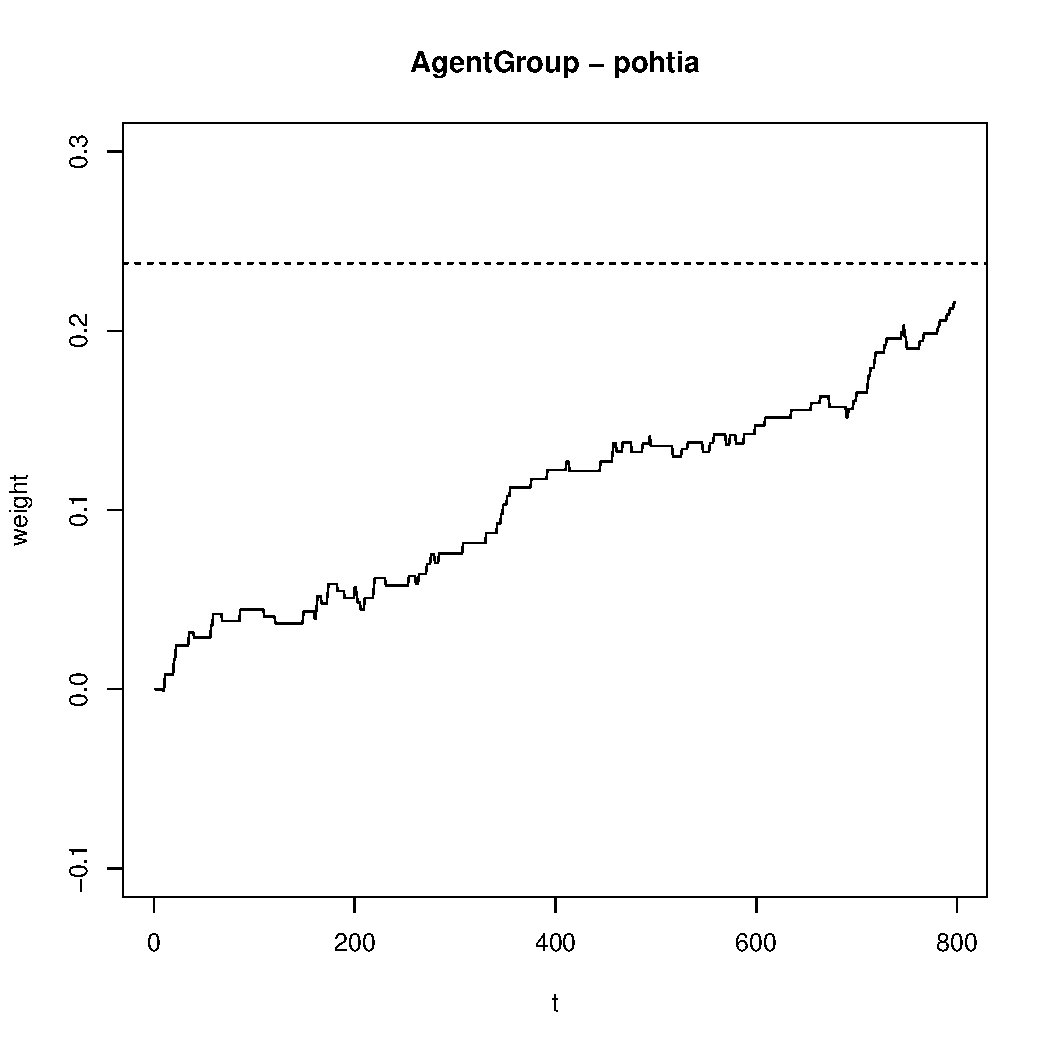
\includegraphics[width=4cm]{{{img/think.qitl1.AgentGroup_pohtia_RW_vs_D}}} &
      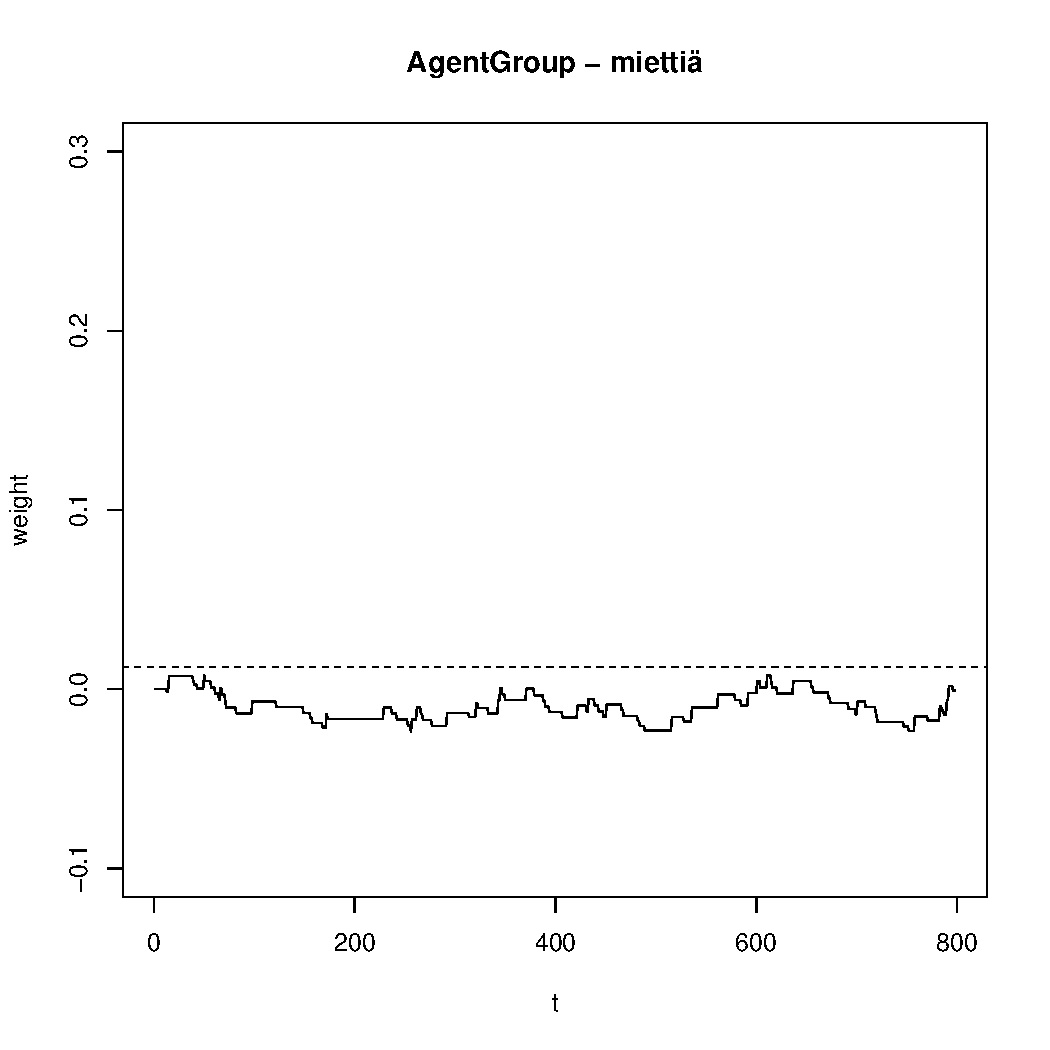
\includegraphics[width=4cm]{{{img/think.qitl1.AgentGroup_miettia_RW_vs_D}}} \\
      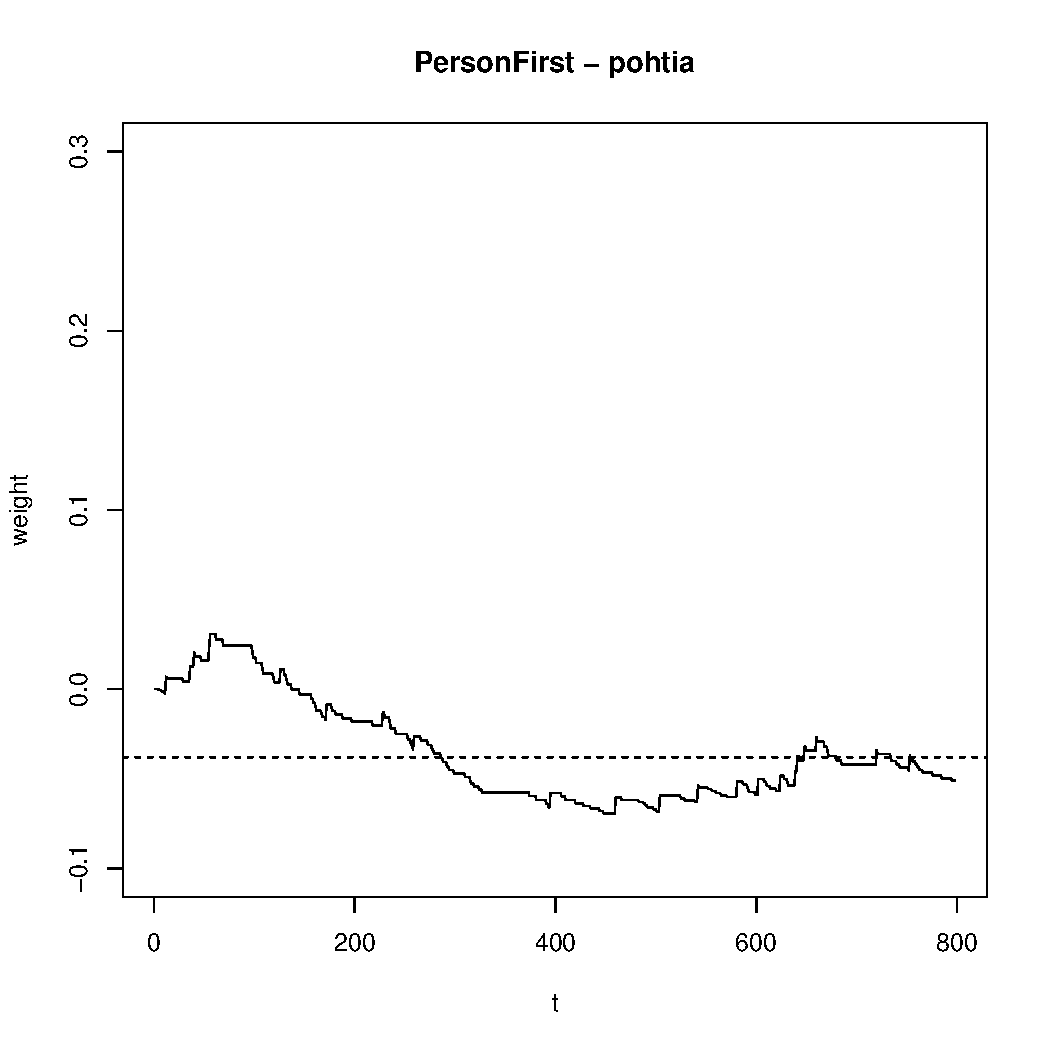
\includegraphics[width=4cm]{{{img/think.qitl1.PersonFirst_pohtia_RW_vs_D}}} &
      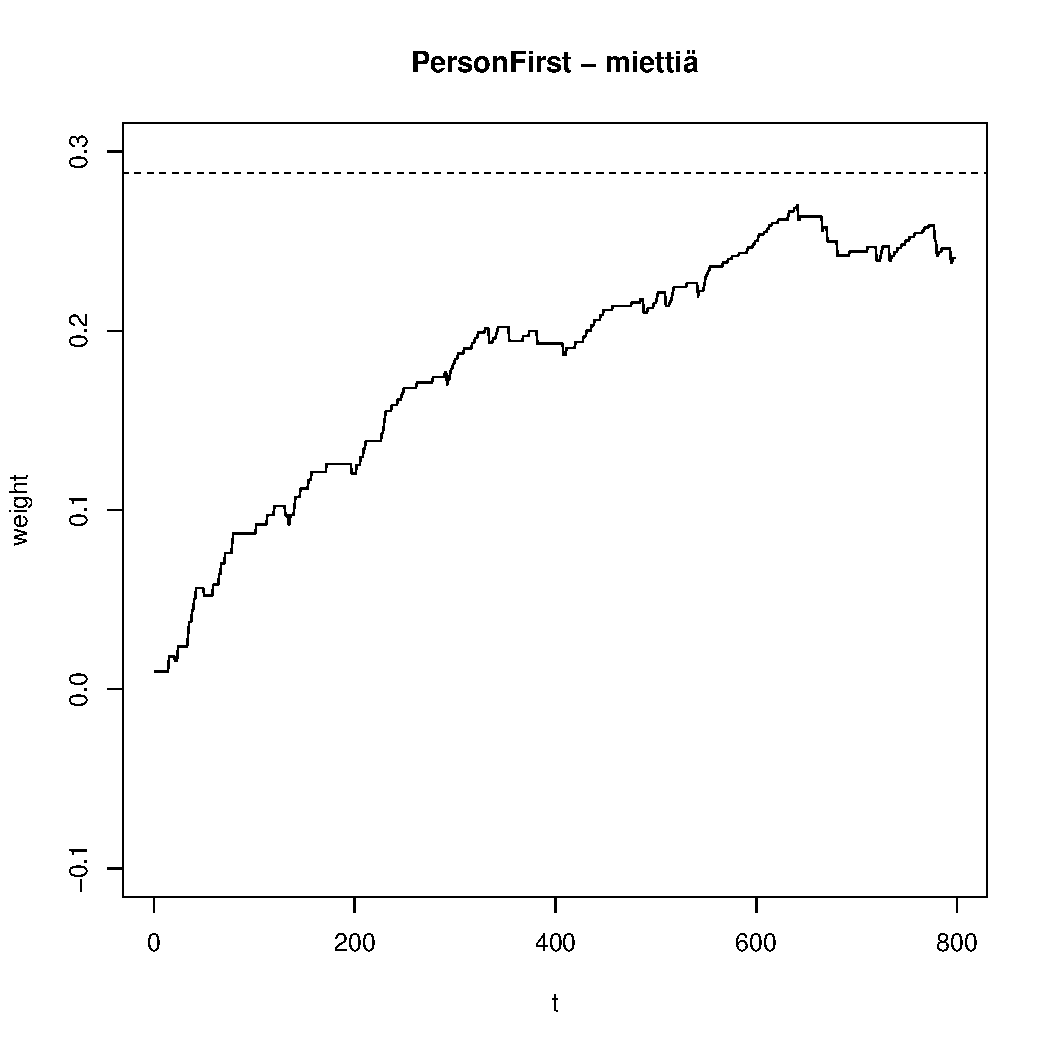
\includegraphics[width=4cm]{{{img/think.qitl1.PersonFirst_miettia_RW_vs_D}}} \\
    \end{tabular}}%
\end{frame}


% \begin{frame}
%   \frametitle{QITL-01: Linguistic production vs. judgments}

%   {\scriptsize
%     \begin{table}[h]
%       \begin{tabular}{ c  c || c || c  c}
%         \hline
%         Forced-choice &               & Frequency  &               & Acceptability \\
%         Dispreferred  & Preferred     & (relative) & Unacceptable  & Acceptable  \\ \hline \hline
%         \multicolumn{1}{c|}{$\varnothing$} & +             & Frequent   & \multicolumn{1}{c|}{$\varnothing$} & +           \\ \hline
%         \multicolumn{1}{c|}{+}             & $\varnothing$ & Rare       & \multicolumn{1}{c|}{+}             & +           \\
%         \hline
%       \end{tabular}
%     \end{table}
%   }
%   $Frequency \Rightarrow Acceptability$ \\
%   $Unacceptability \Rightarrow Rarity$ \\
%   $\neg(Acceptability \Rightarrow Frequency)$ \\
%   $\neg(Rarity \Rightarrow Unacceptability)$ \\
% \end{frame}

\begin{frame}[c]
  \frametitle{QITL-1 through the lens of QITL-6}
  \framesubtitle{(courtesy of Dagmar Divjak)}

  \centering\ungap[2]
  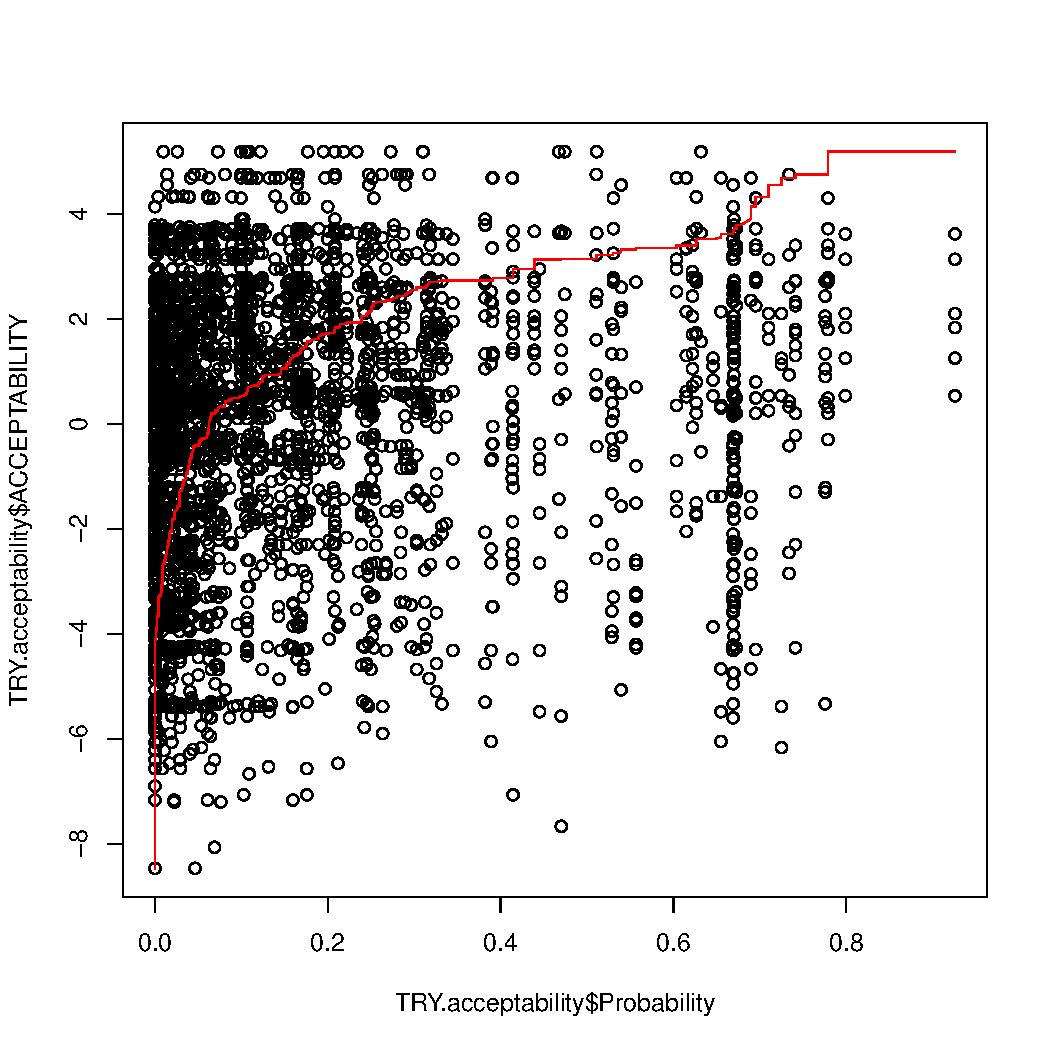
\includegraphics[width=8cm]{{{img/TRY.ACCEPTABILITY_vs_Probability}}}
\end{frame}

\begin{frame}[c]
  \frametitle{Simple \vs complex settings -- QITL-2 revisited}

  \centering
  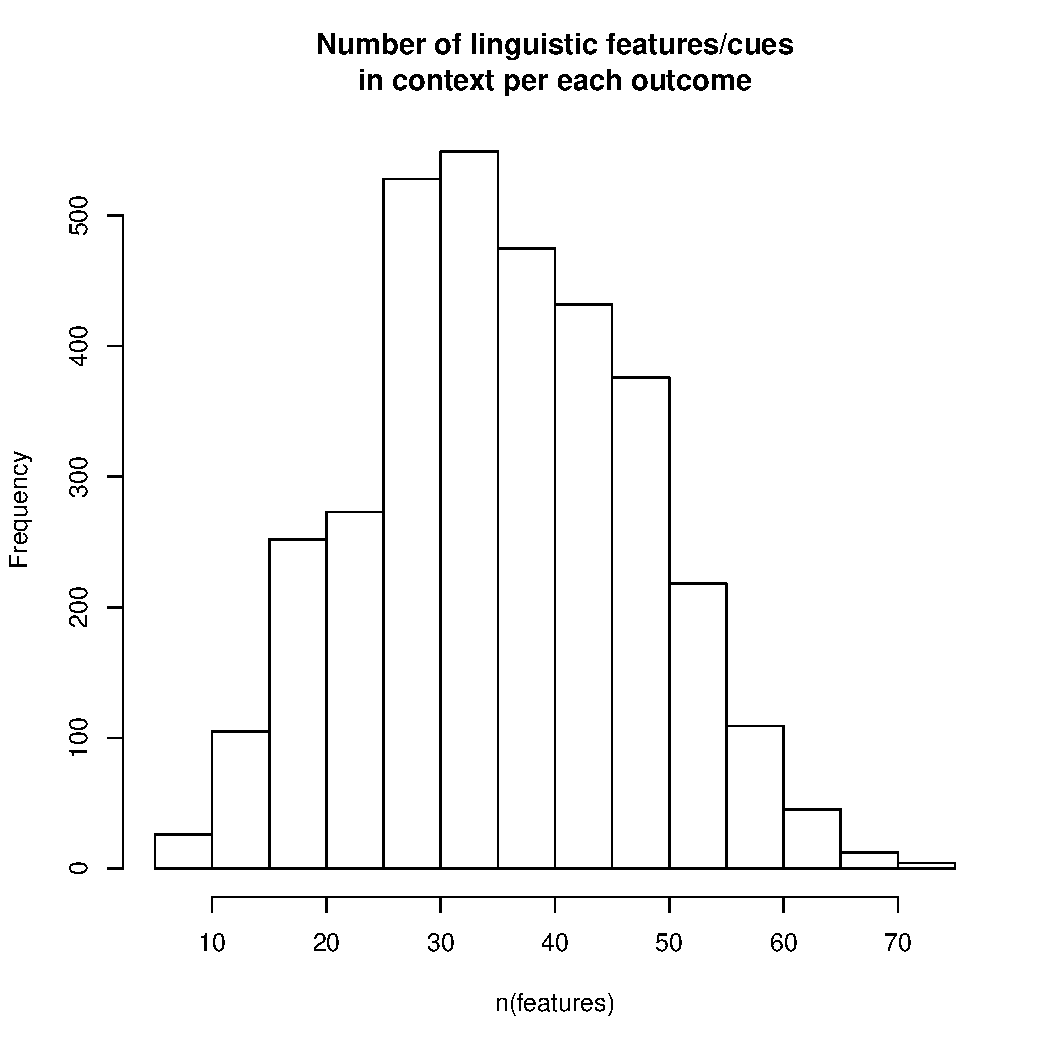
\includegraphics[width=7cm]{{{img/THINK.maximal_linguistic_variable_density}}}
\end{frame}

\begin{frame}
  \frametitle{QITL-4 revisited -- NDL \vs statistical classifiers}

  \begin{center}
    \footnotesize
    \begin{tabular}{lrrr}
      \hline
      & $\lambda_{\mbox{\tiny prediction}}$ & $\tau_{\mbox{\tiny classification}}$ & accuracy \\ 
      \hline
      Polytomous logistic regression & 0.447 & 0.516 & \textbf{0.646} \\ 
      (One-vs-rest) &  &  &  \\ 
      Polytomous mixed logistic regression &  &  &  \\ 
      (Poisson reformulation) &  &  &  \\ 
      $\quad\bullet$ 1$|$Register & 0.435 & 0.505 & 0.638 \\ 
      $\quad\bullet$ 1$|$Genre & 0.433 & 0.504 & 0.637 \\ 
      $\quad\bullet$ 1$|$Lexeme & 0.428 & 0.499 & 0.634 \\ 
      $\quad\bullet$ 1$|$Register + 1$|$Lexeme & 0.431 & 0.502 & 0.636 \\ 
      Support Vector Machine & 0.414 & 0.487 & 0.625 \\ 
      Memory-Based Learning & 0.287 & 0.376 & 0.543 \\ 
      (TiMBL) &  &  &  \\ 
      Random Forests & 0.445 & 0.515 & \textbf{0.645} \\ 
      Naive Discriminative Learning & 0.442 & 0.511 & \primary{0.642} \\ 
      \hline
    \end{tabular}
  \end{center}
  
  \scriptsize
  \secondary{Table:} Classification diagnostics for models fitted to the English data set ($n=909$). 
\end{frame}

%%% Local Variables: 
%%% mode: latex
%%% TeX-master: "../qitl6_evert_arppe"
%%% End: 
